\documentclass[10pt]{beamer}

\usetheme{metropolis}
\usepackage{appendixnumberbeamer}
\usepackage{pgfbaseimage}
\usepackage{booktabs}
\usepackage[scale=2]{ccicons}

\usepackage{pgfplots}	
\usepgfplotslibrary{dateplot}

\usepackage{xspace}
\usepackage[spanish]{babel}
\usepackage[utf8]{inputenc}
%videos
\usepackage{multimedia}
%\usepackage{animate,media9,movie15}
\newcommand{\themename}{\textbf{\textsc{metropolis}}\xspace}
\pgfdeclareimage[width=5cm,height=3cm]{loralogo}{imagenes/loralogo.png} 
\newcommand{\tab}[1]{\hspace{.2\textwidth}\rlap{#1}}

\title{Defensa de título:}
\subtitle{\normalsize Diseño y evaluación de simulador de dispositivos LoRaWAN Gateway\\junto a la implementación de un sistema de transición a IPv6}
\date{\today}
\author{Víctor Manríquez	 Gallegos\\
\newline
\scriptsize
Profesor Guía:Diego Dujovne\\
Comité: José Pérez\\
\phantom{x}\hspace{7.5ex}Nicolás Boettcher }
\institute{Universidad Diego Portales}
\titlegraphic{\hfill
\includegraphics[scale=0.3]{imagenes/eit}}

\begin{document}

\maketitle

\begin{frame}{Tabla de Contenidos}
  \setbeamertemplate{section in toc}[sections numbered]
  \tableofcontents[hideallsubsections]
\end{frame}

\section{LoRaWAN}

\begin{frame}[fragile]{LoRaWAN}
\begin{itemize}
\item ¿Qué es?
\item Requisitos de funcionamiento
\item Tipos de dispositivos
\item Arquitectura de red para LoRaWAN
\item ALOHAnet
\item Características de dispositivos LoRa
\item Fases de comunicación
\end{itemize}
\end{frame}

\begin{frame}[fragile]{¿Qué es?}
\begin{figure}
\begin{overprint}
\hspace{2cm}\onslide<1>\centering
\includegraphics[scale=0.8]{imagenes/loralogo}\caption{Logo LoRa}
\end{overprint}
\end{figure}
\end{frame}

\begin{frame}[fragile]{Requisitos de funcionamiento}
\begin{figure}
\onslide<1>\centering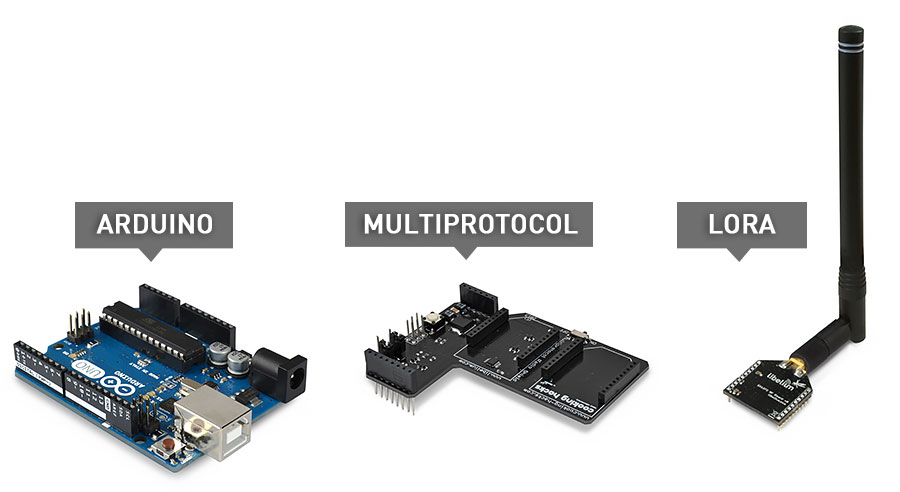
\includegraphics[scale=0.3]{imagenes/lora1}\caption{Composición dispositivo LoRa + Arduino}
\end{figure}
\end{frame}

\begin{frame}[fragile]{Tipos de dispositivos}
\begin{figure}
\begin{overprint}
\onslide<1>\centering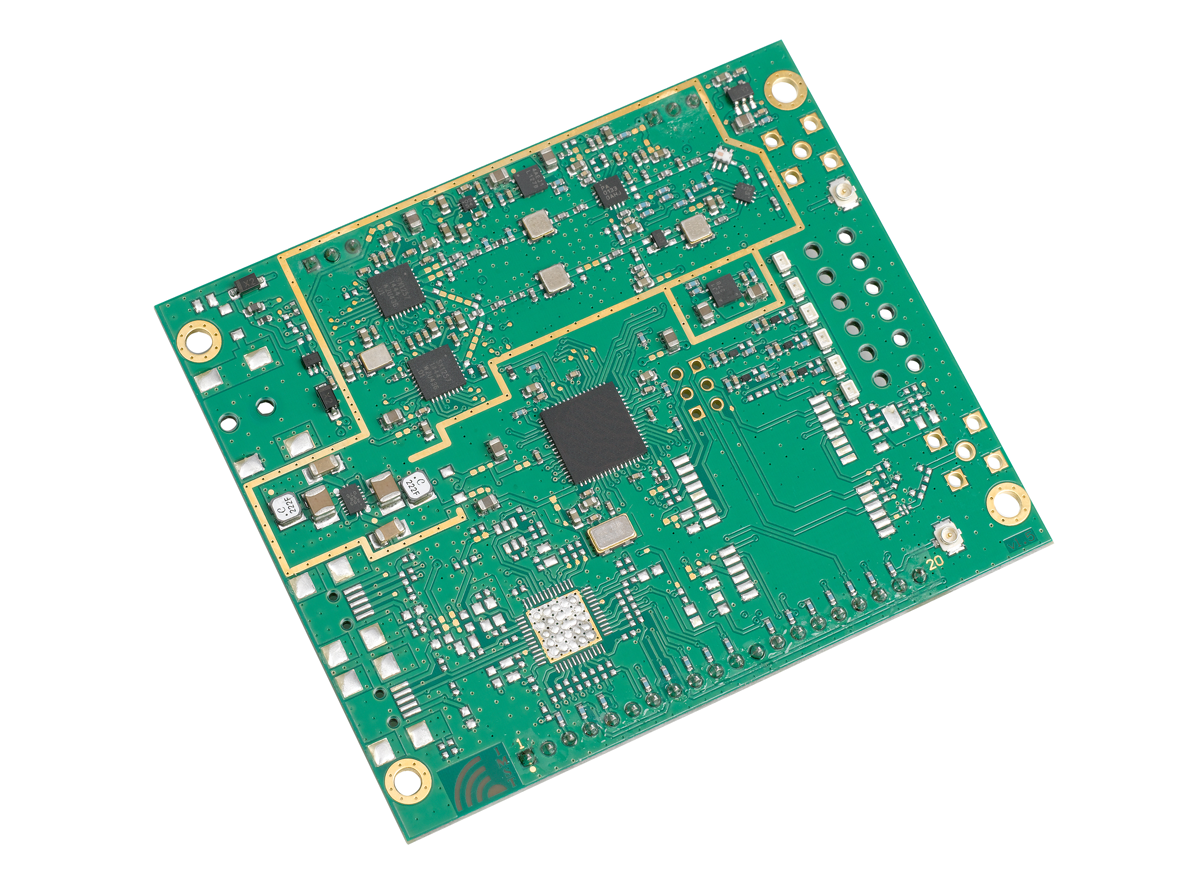
\includegraphics[scale=0.2]{imagenes/concentrador}\caption{Concentrador LoRa IC880A}
\onslide<2>\centering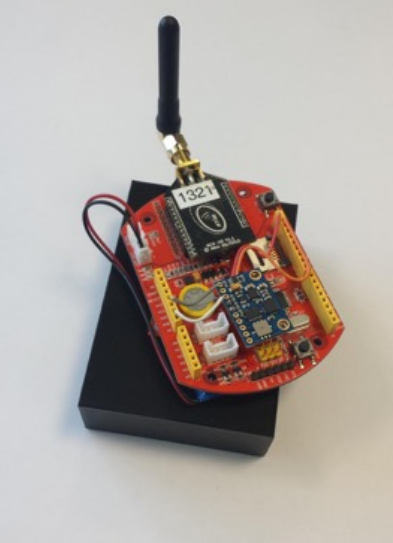
\includegraphics[scale=0.3]{imagenes/lora}\caption{Nodo LoRa inAir9}
\hspace{2cm}\onslide<3>\centering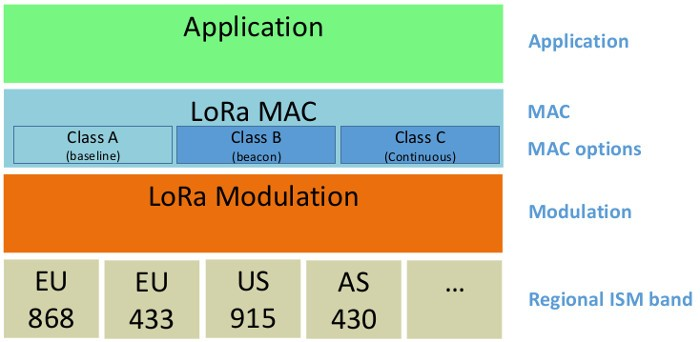
\includegraphics[scale=0.4]{imagenes/capaslora}\caption{Arquitectura de capas}
\end{overprint}
\end{figure}
\end{frame}
%
\begin{frame}[fragile]{ALOHAnet}
\begin{itemize}
\item Sistema de comunicación inalámbrica de dispositivos
\item Dos canales de comunicación (envío/recepción)
\item Envío y recepción de mensajes en ventanas de tiempo
\item Variante de ALOHA, permite programación de mensajes
\end{itemize}
\end{frame}
%%
%arqui de red
%%
\begin{frame}[fragile]{Arquitectura de red para LoRaWAN}
\begin{figure}
\centering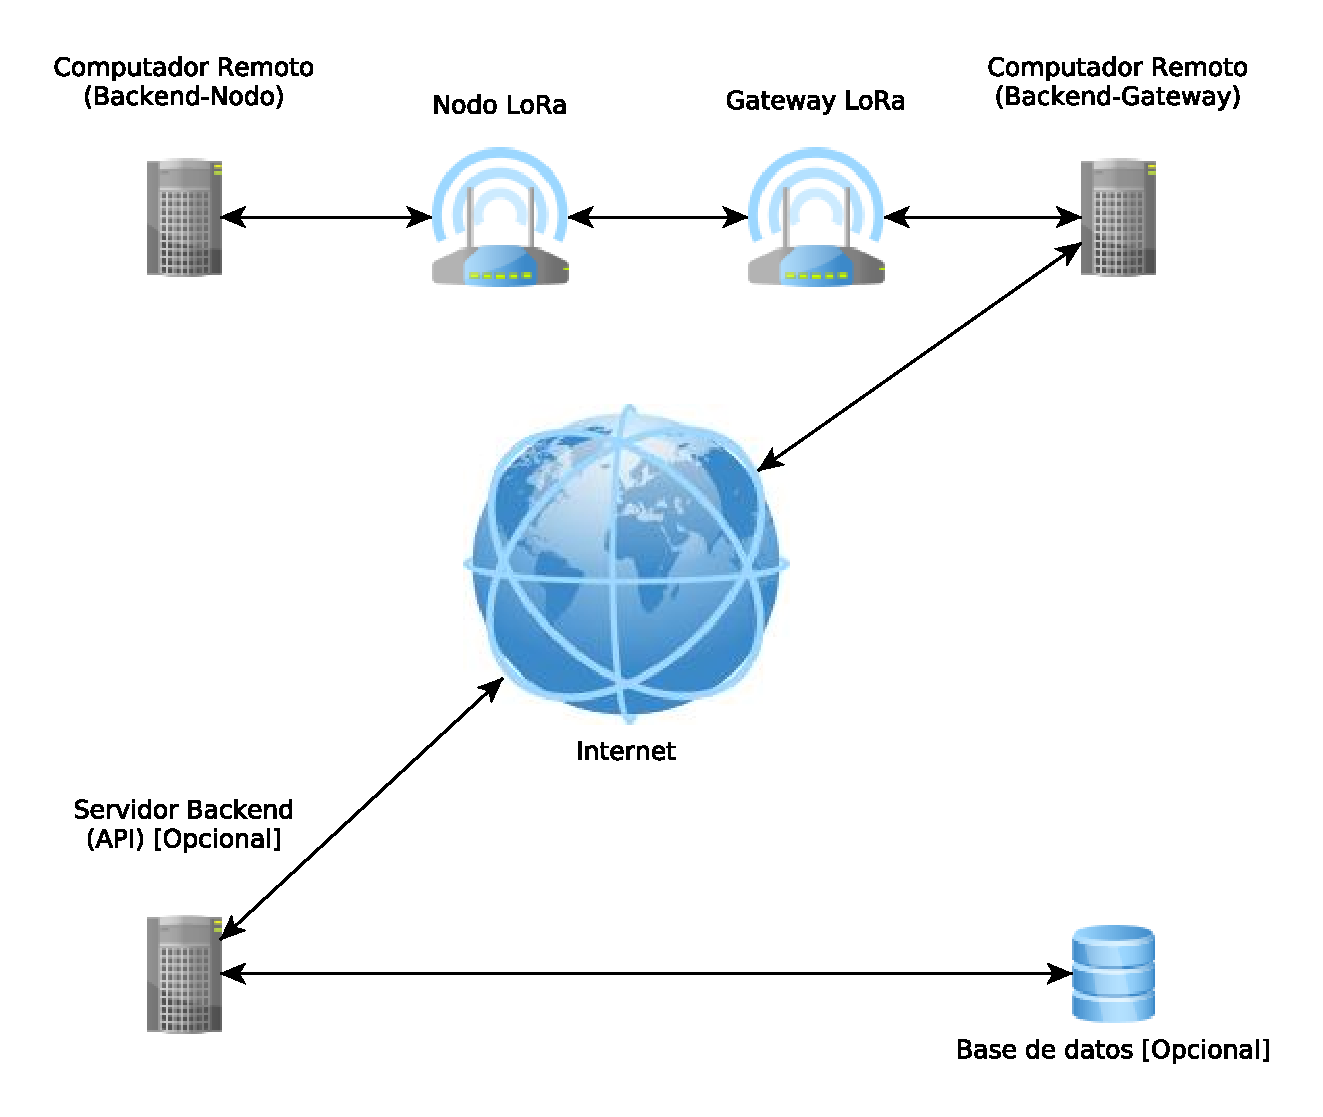
\includegraphics[scale=0.37]{imagenes/arquilora.eps}\caption{Arquitectura de red para LoRaWAN}
\end{figure}
\end{frame}
%%

\begin{frame}[fragile]{Características de los dispositivos LoRa}
\begin{itemize}
\item Espectro expandido de señal
\begin{itemize}
\item Multi-canal
\item Protección contra interferencias
\end{itemize}
\item Listen before talk
\item Tasa de envío adaptable (ADR)
\item Topología estrella-de-estrellas
\end{itemize}
\end{frame}

\begin{frame}[fragile]{Fases de comunicación}
\begin{itemize}
\item Fase de emparejamiento
\item Fase de transmisión
\begin{itemize}
\item Fase de retransmisión
\end{itemize}
\item Fase de reposo
\end{itemize}
\end{frame}

\section{Módulo de transición}
\begin{frame}[fragile]{Módulo de transición}
\begin{itemize}
\item Funcionamiento
\item Aportes
\end{itemize}
\end{frame}

\begin{frame}[fragile]{Funcionamiento}
\begin{figure}
\begin{overprint}
\onslide<1>\centering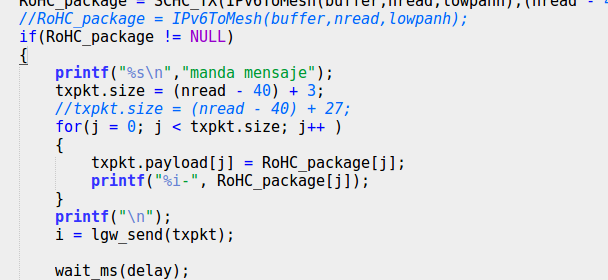
\includegraphics[scale=0.5]{imagenes/codigo1}\caption{Código de módulo de transición, integrado a código de Semtech (1/3)}
\onslide<2>\centering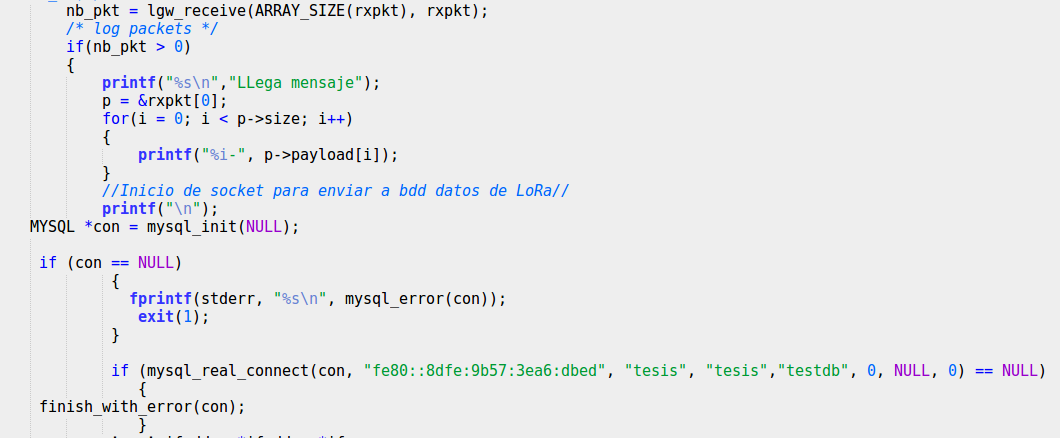
\includegraphics[scale=0.3]{imagenes/codigo2}\caption{Código de módulo de transición, integrado a código de Semtech (2/3)}
\onslide<3>\centering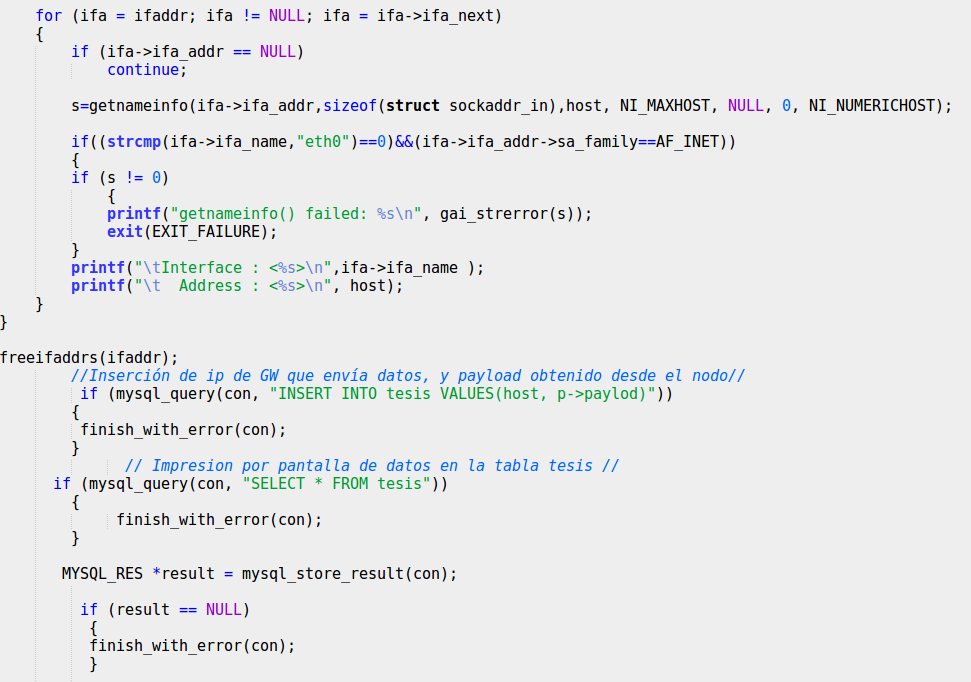
\includegraphics[scale=0.3]{imagenes/codigo3}\caption{Código de módulo de transición, integrado a código de Semtech (3/3)}
\end{overprint}
\end{figure}
\end{frame}

\begin{frame}[fragile]{Aportes}
\begin{itemize}
\item Middleware para comunicación entre LoRaWAN e IPv6
\item Posibilidad de agregar protocolos criptográficos como SSL o TLS
\item Métodos de extracción de datos desde cabecera de paquete LoRaWAN
\end{itemize}
\end{frame}
\section{Simulador}

\begin{frame}[fragile]{Simulador}
\begin{itemize}
\item Fases de comunicación
\item Resultados Obtenidos
\item Demostración
\end{itemize}
\end{frame}

\begin{frame}[fragile]{Fase de emparejamiento}
\begin{figure}
\centering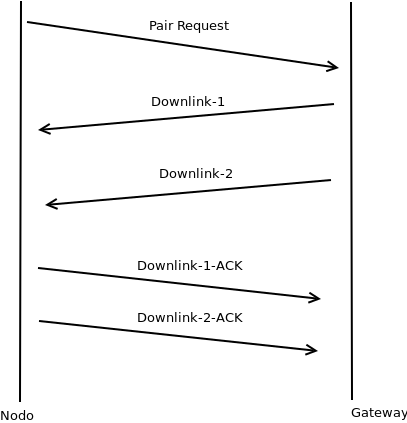
\includegraphics[scale=0.37]{imagenes/pair}\caption{Diagrama de flujo de mensajes en fase de emparejamiento}
\end{figure}
\end{frame}

\begin{frame}[fragile]{Fase de transmisión}
\begin{figure}
\begin{overprint}
\onslide<1>\centering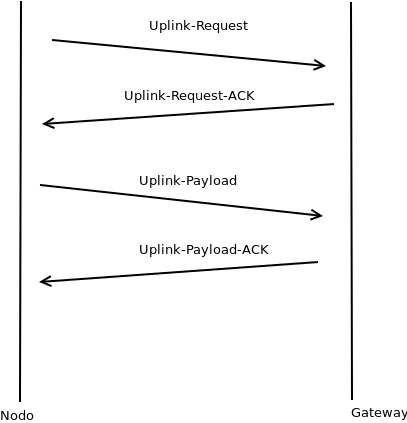
\includegraphics[scale=0.37]{imagenes/transmit}\caption{Diagrama de flujo de mensajes en fase de transmisión}
\onslide<2>\centering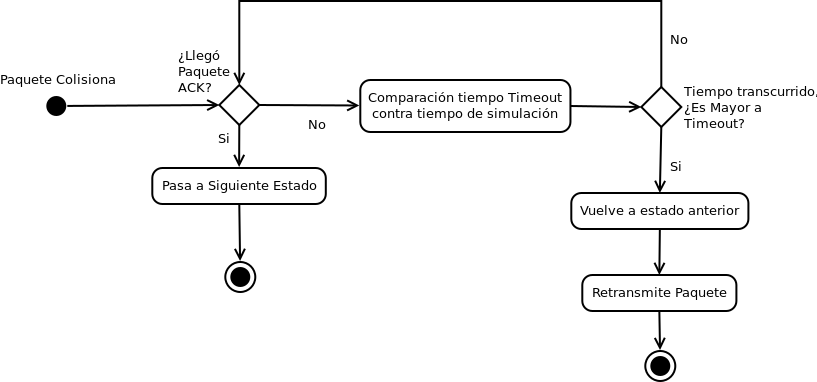
\includegraphics[scale=0.37]{imagenes/retrans}\caption{Diagrama de flujo que representa fase de retransmisión}
\end{overprint}
\end{figure}
\end{frame}

\begin{frame}[fragile]{Resultados Obtenidos}
\begin{figure}
\begin{overprint}
\onslide<1>\centering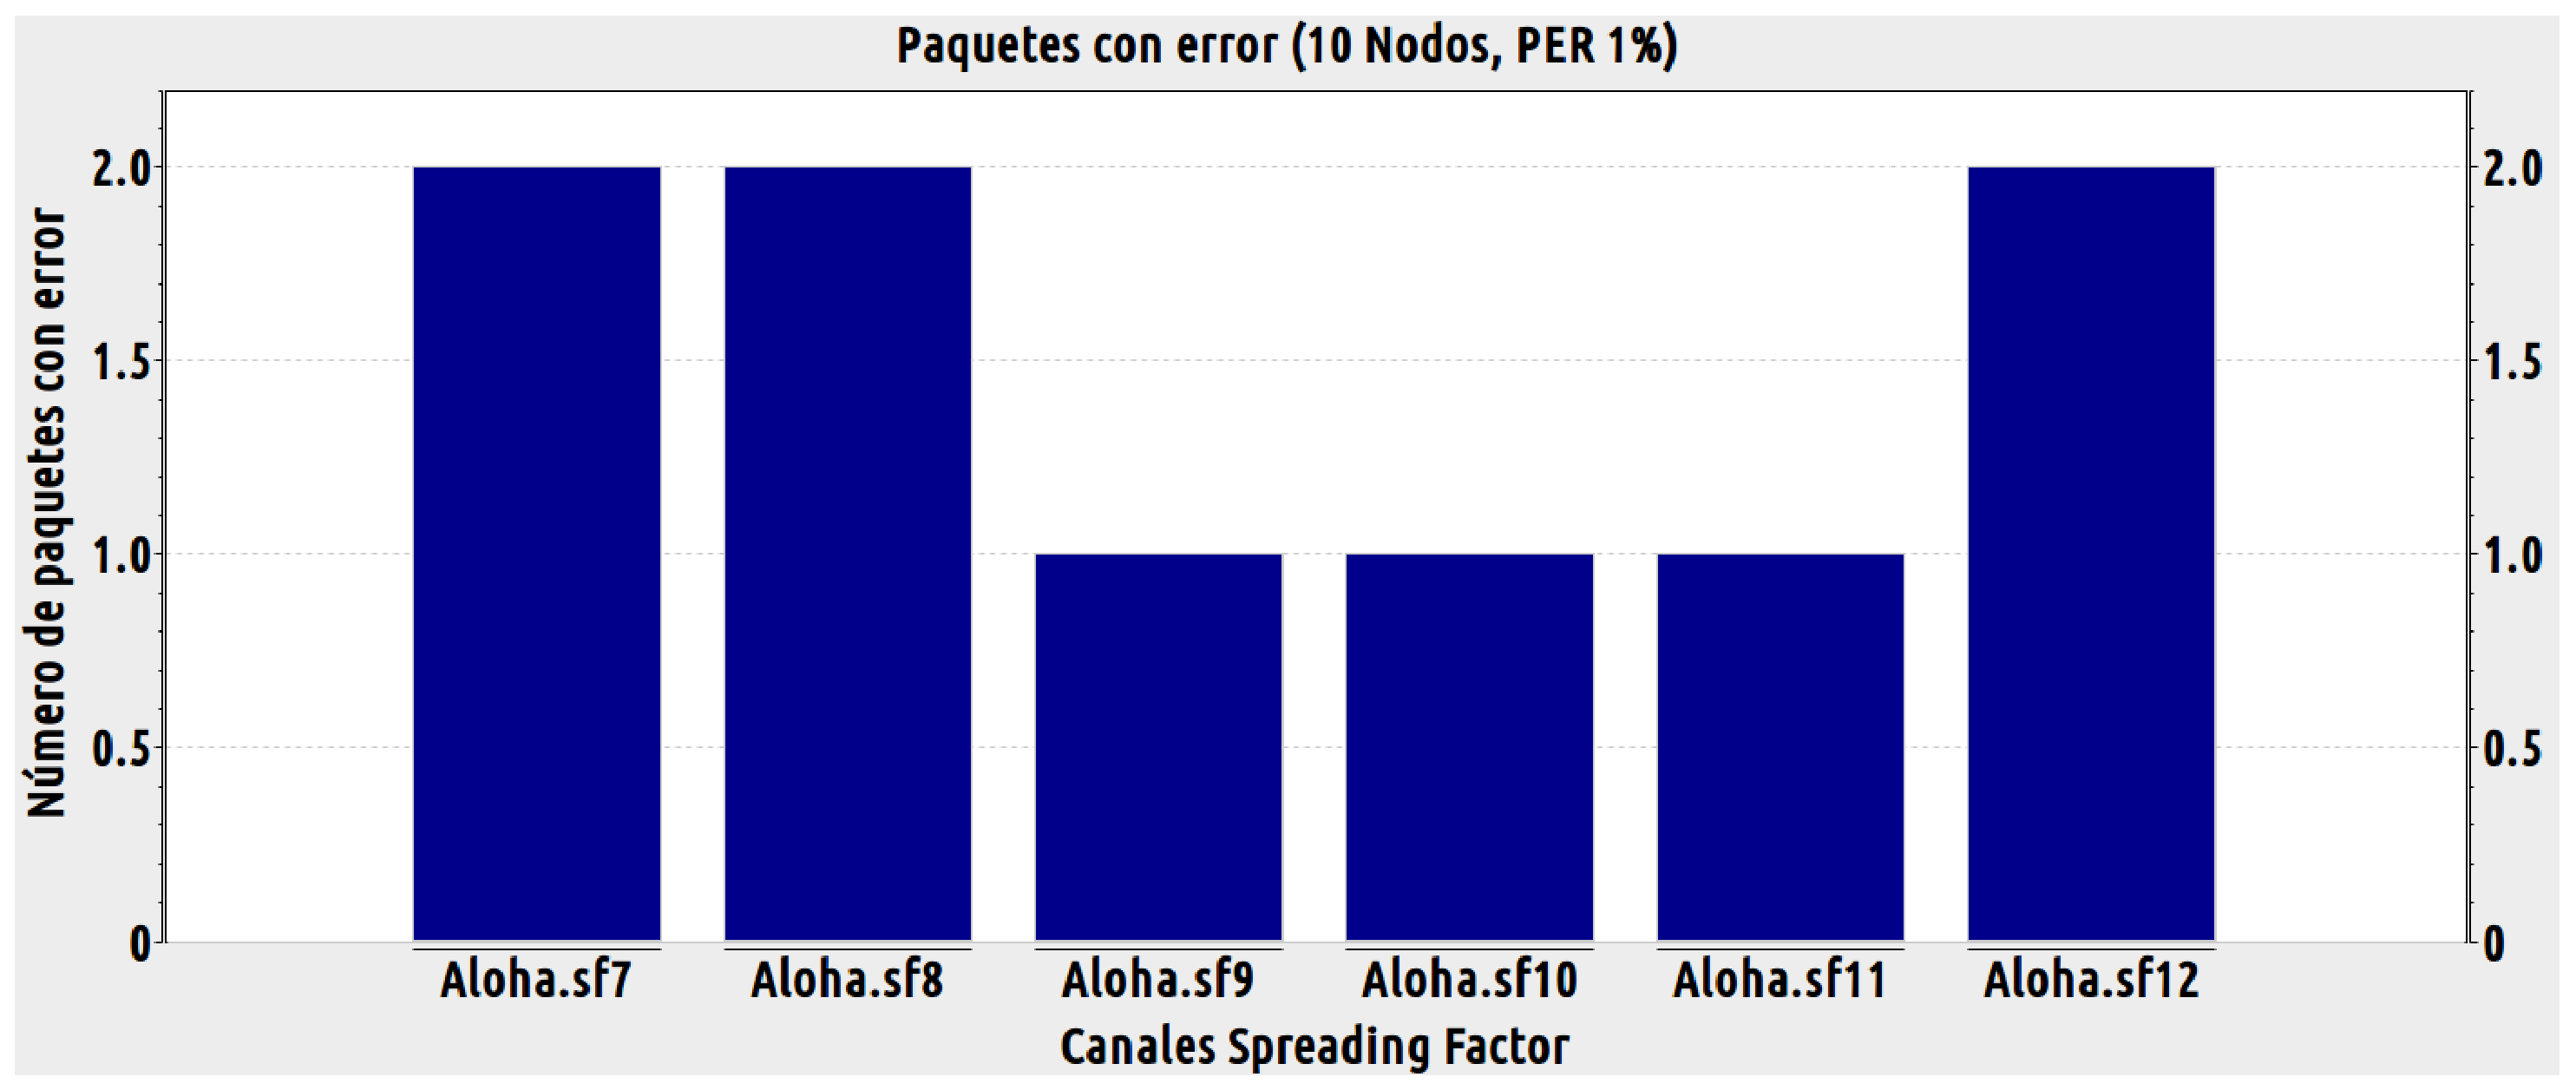
\includegraphics[scale=0.2]{imagenes/errores10nodos.eps}\caption{Gráfico de cantidad de paquetes con errores en cada SF en la simulación para 10 nodos.}
\onslide<2>\centering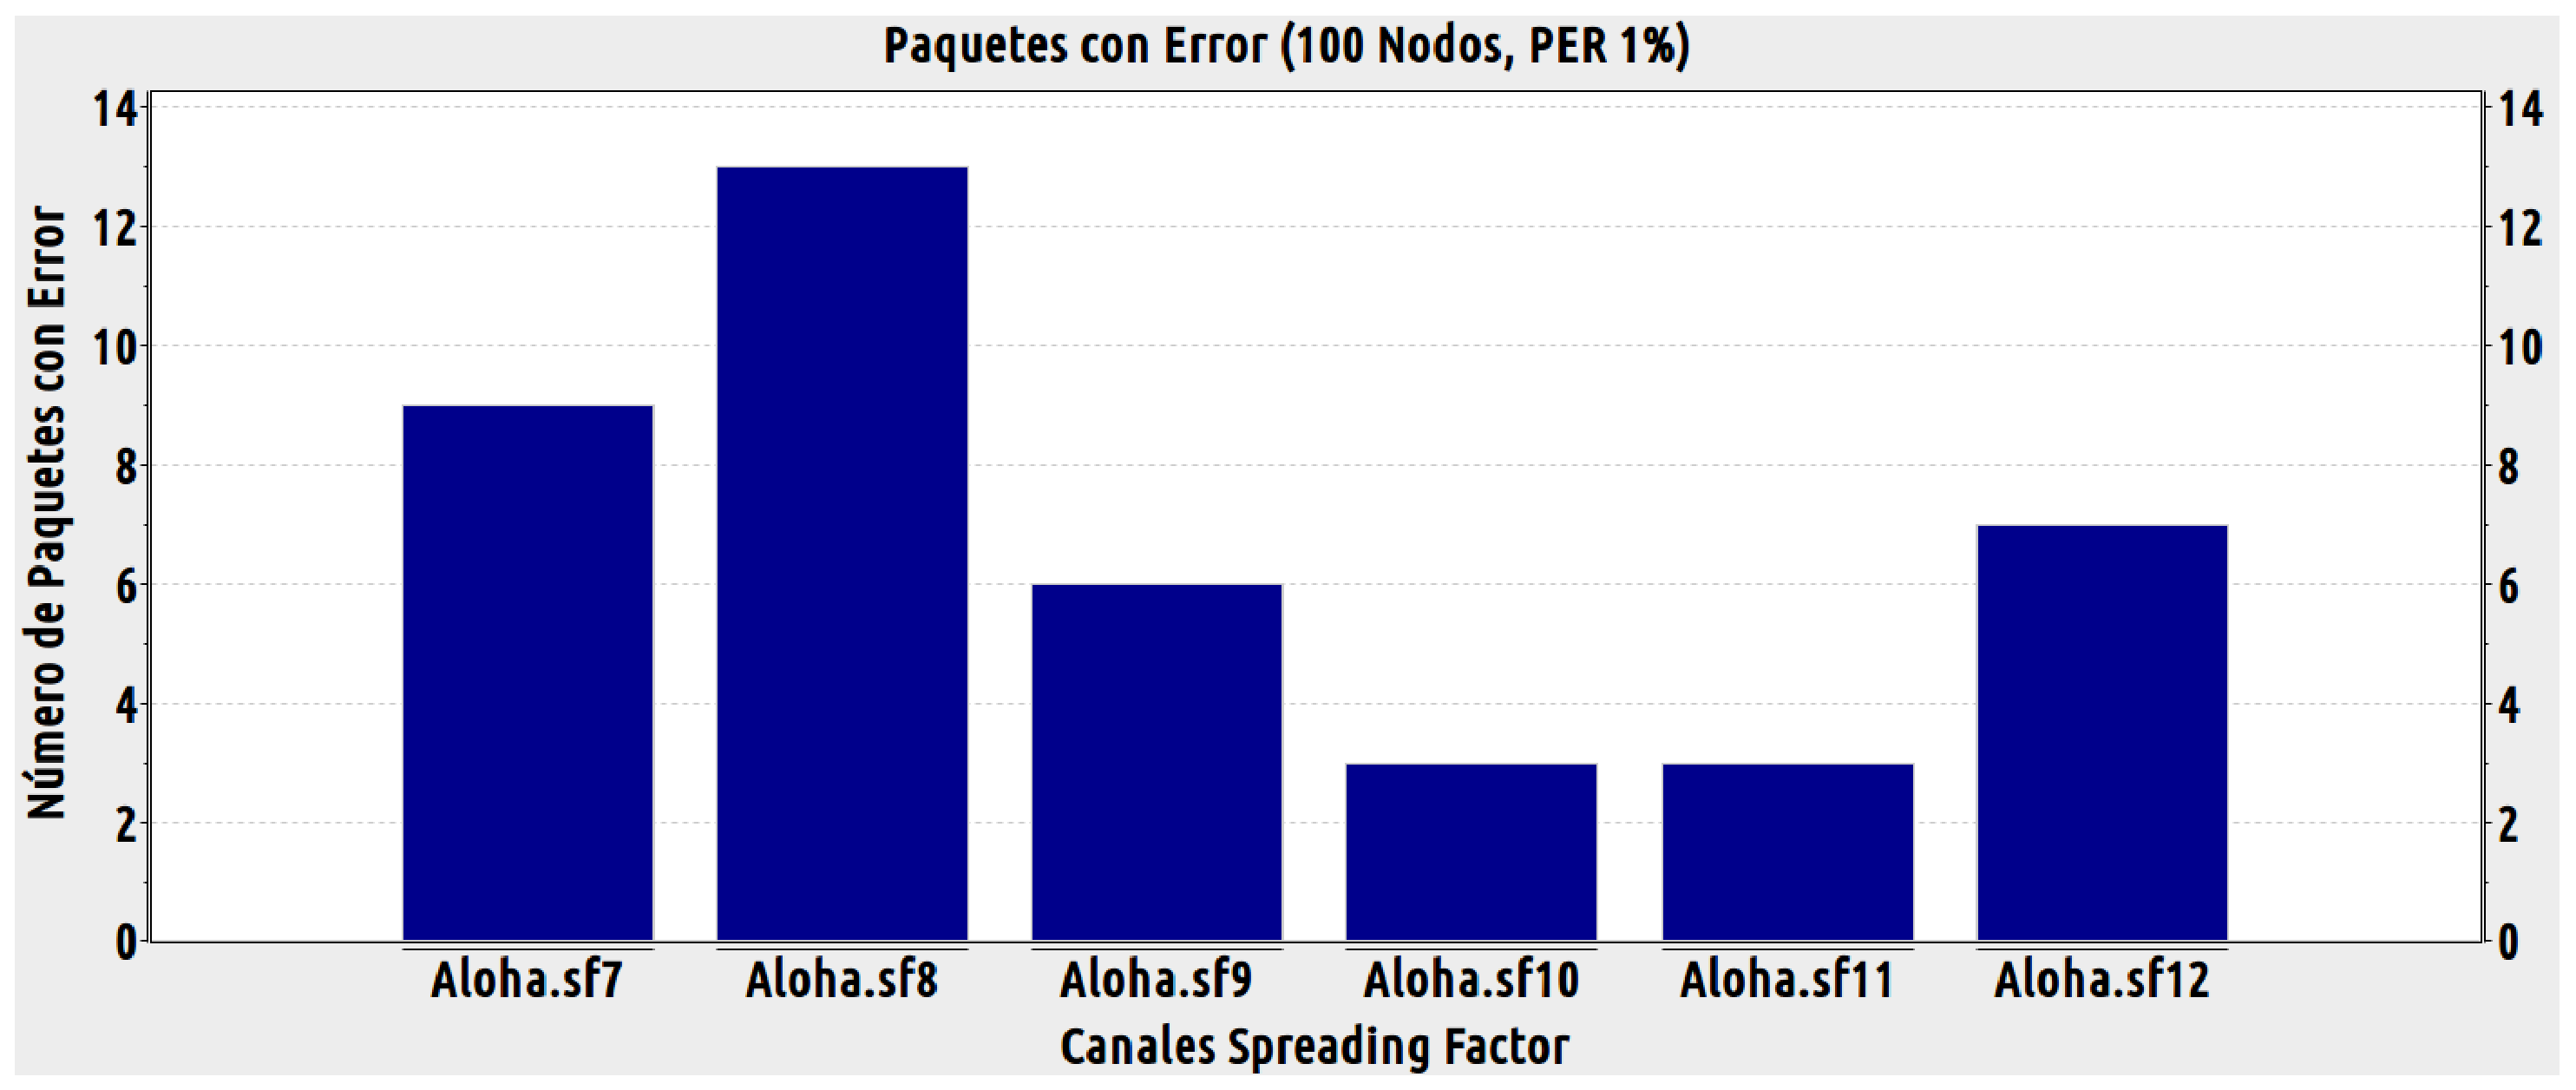
\includegraphics[scale=0.2]{imagenes/errores100nodos.eps}\caption{Gráfico de cantidad de paquetes con errores en cada SF en la simulación para 100 nodos.}
\onslide<3>\centering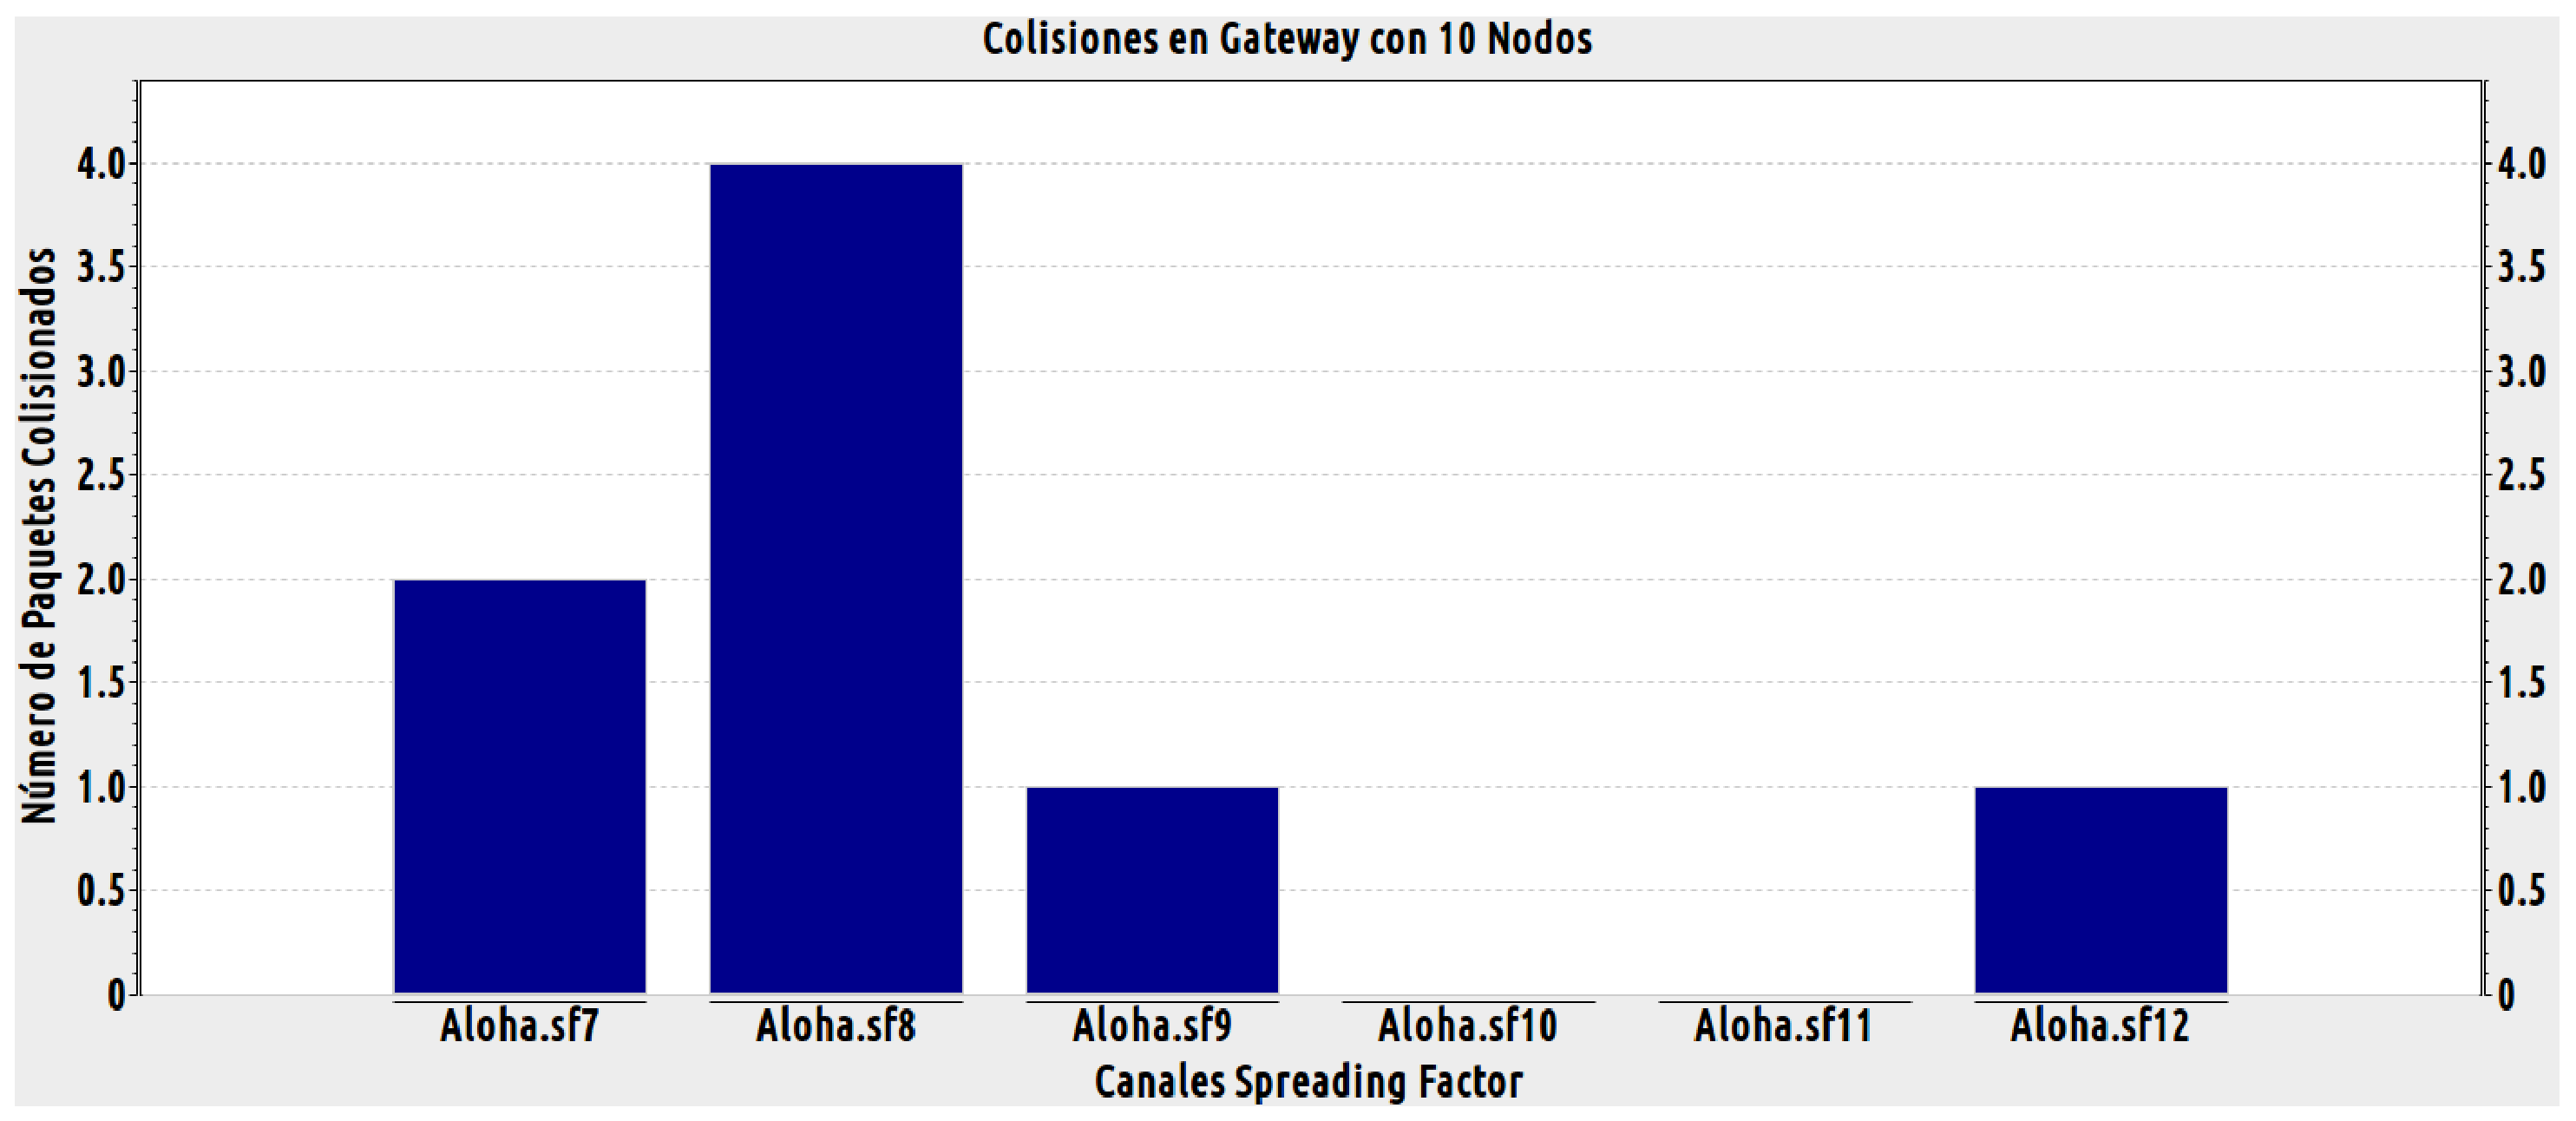
\includegraphics[scale=0.2]{imagenes/colisiones10nodos.eps}\caption{Gráfico de cantidad de paquetes colisionados en cada SF en la simulación con 10 nodos.}
\onslide<4>\centering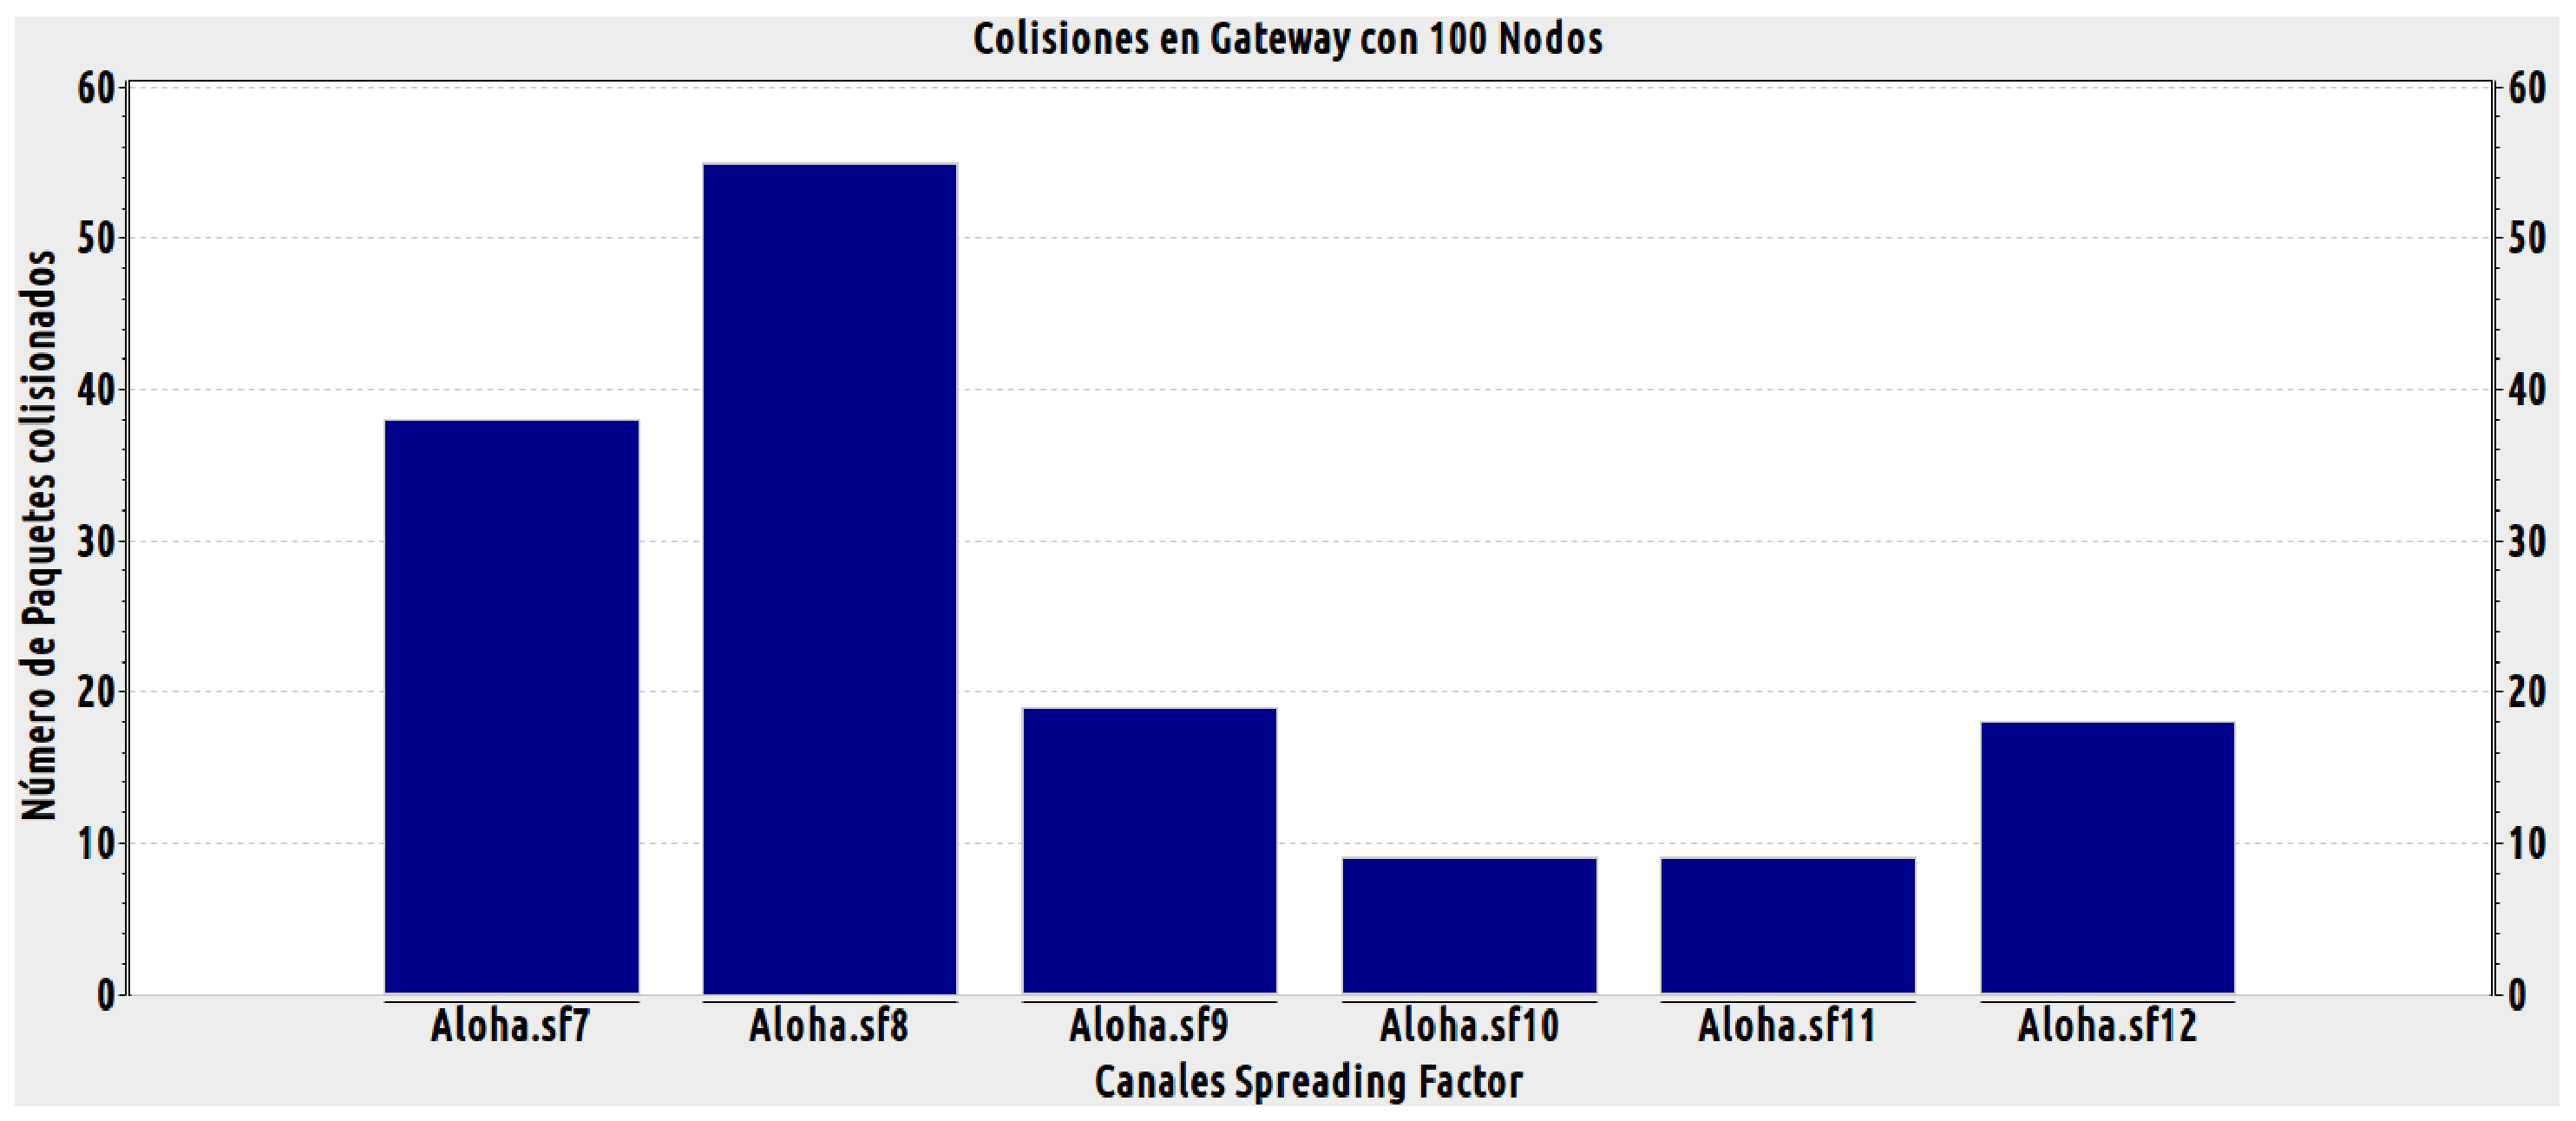
\includegraphics[scale=0.2]{imagenes/colisiones100nodos.eps}\caption{Gráfico de cantidad de paquetes colisionados en cada SF en la simulación con 100 nodos.}
\end{overprint}
\end{figure}
\end{frame}

\begin{frame}[fragile]{Demostración}

\centering\movie[externalviewer, height = 0.6\textwidth, width = 1.0\textwidth, poster, showcontrols]{\pgfuseimage{loralogo}}{video/10nodos.mp4}
 
%\movie[externalviewer,showcontrols=true,width=10cm,height=8cm]{\pgfuseimage{loralogo}}{video/10nodos.mkv}
\end{frame}

\section{Conclusiones}
\begin{frame}[fragile]{Conclusiones}
\begin{itemize}
\item Simulador logró un comportamiento análogo a nivel lógico
\item Se logró agregar componentes reales de pérdida al simulador
\item Módulo de transición permite correcto envío de información desde red LoRa a red IPv6
\end{itemize}
\end{frame}

\begin{frame}[standout]
  ¿Preguntas?
\end{frame}

\appendix

\begin{frame}[fragile]{Preguntas}
\begin{figure}
\begin{overprint}
\onslide<1>\centering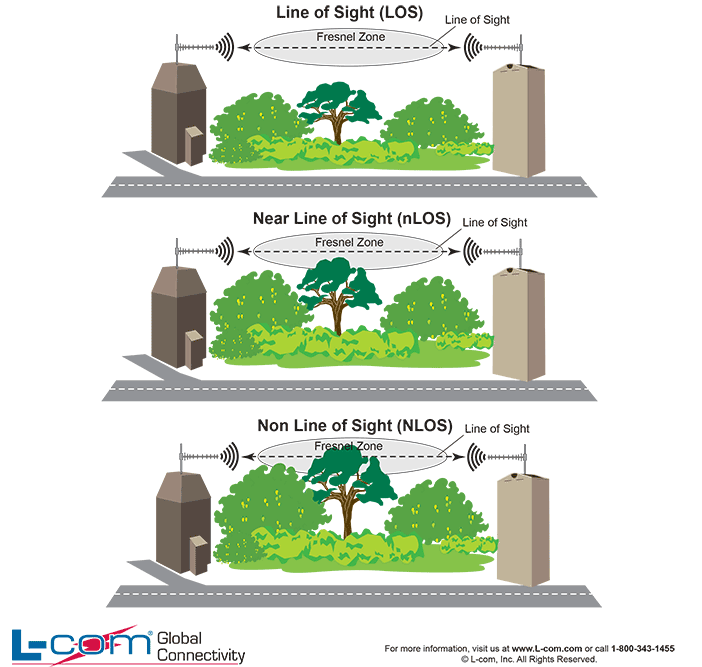
\includegraphics[scale=0.3]{imagenes/los}\caption{Imagen que representa comunicación por Línea de Vista}
\onslide<2>\centering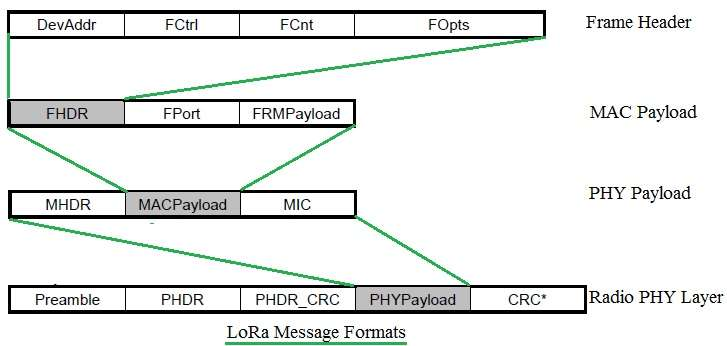
\includegraphics[scale=0.4]{imagenes/msg}\caption{Imagen que representa estructura de mensaje en protocolo LoRaWAN}
\end{overprint}
\end{figure}
\end{frame}

\end{document}
